\documentclass[a4paper,11pt,fleqn]{article}%fleqn pour aligner les equations à gauche
\usepackage{../../Styles/Cours}


\newcommand{\chnum}{Chapitre 12}
\newcommand{\chtitle}{Mouvement dans un champ électrique uniforme}
\newcommand{\dtype}{TP}
  
  \begin{document}
  
  \maketitle
  
  \section{Déviation d'un faisceau d'électrons}
 \begin{minipage}{.8\textwidth}
 \begin{enumerate}
  	\item Visionner la vidéo
  	\item Les électrons sont-ils déviés vers la plaque positive ou négative ?
  	\item Quel paramètre expérimental modifie-t-on pour faire varier la déviation du faisceau ? 
\end{enumerate}
\end{minipage} 
\begin{minipage}{.2\textwidth}
	
\includegraphics[scale=1.2]{Ressources/TSPE_C5_Act1_Fig 1.png}
\end{minipage}
  
\section{Forces en présence}
Un électron de masse $m_e$ = \SI{9.1E-31}{kg} et de charge $q$ = $-e$ = \SI{-1,60E-19}{C}, pénètre entre les deux plaques chargées d'un condensateur plan où règne un champ électrique $\vec{E} = E\cdot \vec{k}$ avec $E = \SI{1,6 E4}{\volt\per\meter}$.
\begin{enumerate}\setcounter{enumi}{3} \item Calculer le poids d'un électron et la force électrostatique à laquelle l'électron est soumis. Commenter \end{enumerate}

\section{Les débuts de l'électron - Liban 2014}

 \begin{tabular}{m{3cm} m{10cm} m{3cm}}
 \multicolumn{2}{m{14cm}}{Le problème posé par la nature des "rayons cathodiques'' à la fin du ${19}^{ \text{ème}}$ siècle fut résolu en 1897 par l'anglais J. J. Thomson : il s'agissait de particules chargées négativement baptisées par la suite ``électron''. La découverte de l'électron valut à Thomson le prix Nobel de physique en 1906.} & 
 	\begin{itemize**} 
 		\item  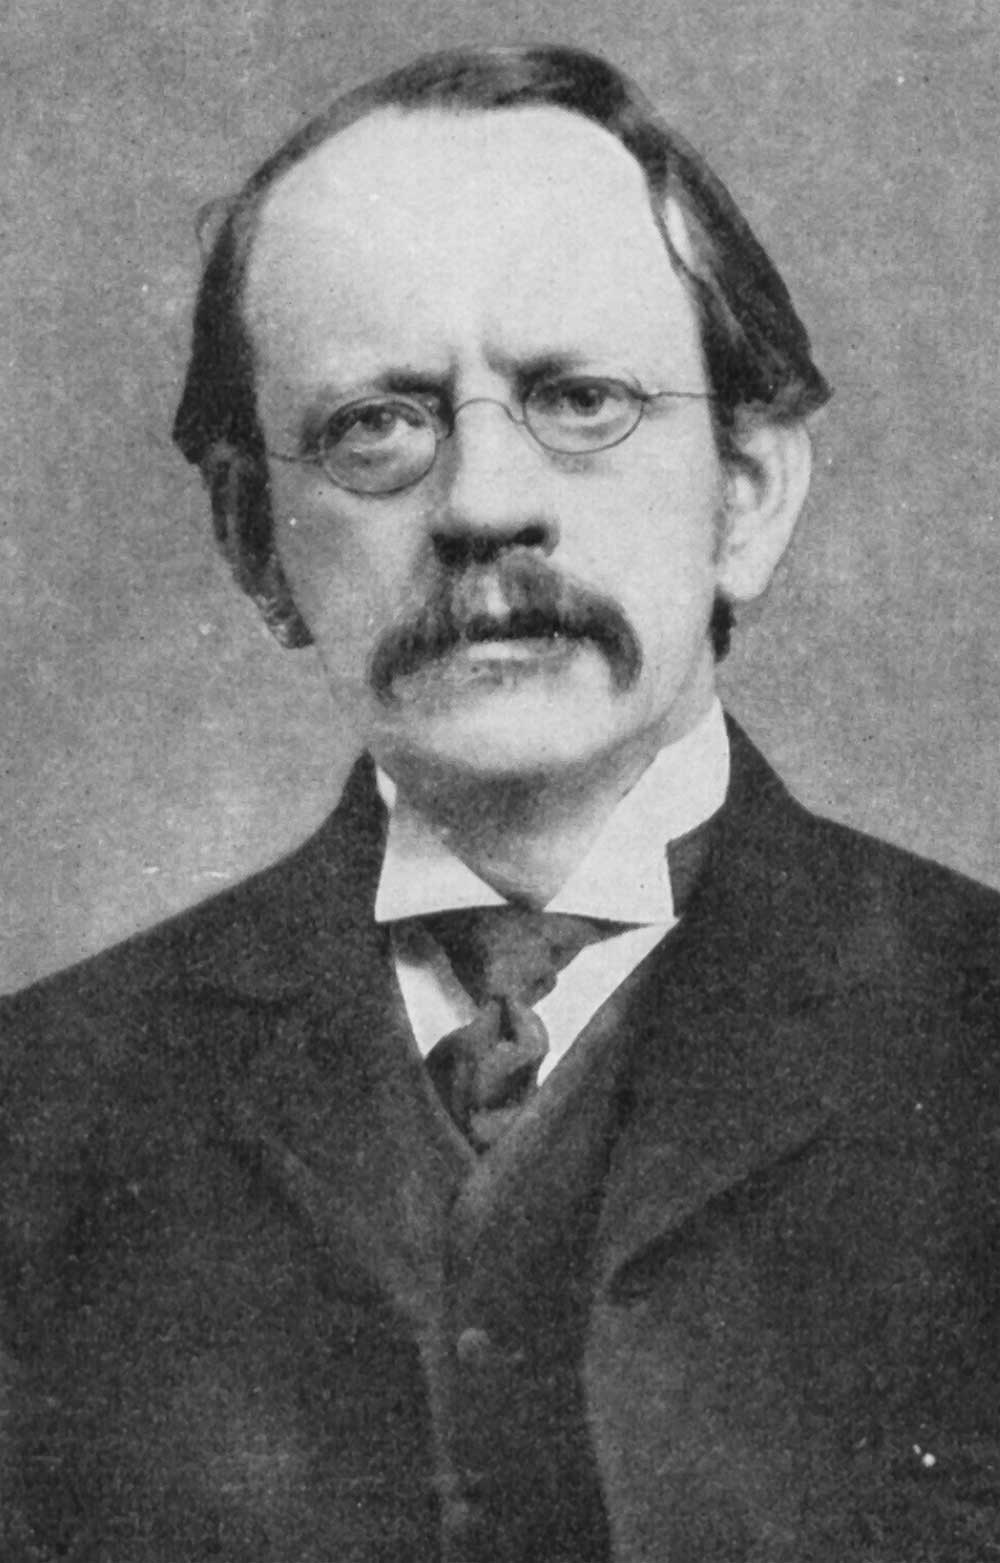
\includegraphics[scale=.07]{Ressources/J.J_Thomson.jpg} 
 		\item J.J. Thomson 
 	\end{itemize**} \\
 
 \multicolumn{3}{m{18cm}}{Le défi pour les scientifiques de l'époque fut alors de déterminer les caractéristiques de cette particule : sa charge électrique et sa masse. Dans un premier temps, Thomson lui-même, en étudiant la déviation d'un faisceau d'électrons dans un champ électrique, put obtenir le rapport $\dfrac{e}{m_e}$.} \\
 
 	\begin{itemize**} 
 		\item  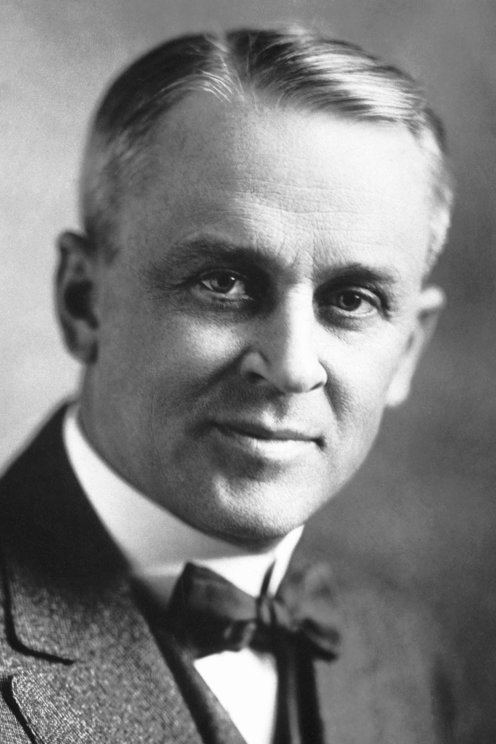
\includegraphics[scale=.8]{Ressources/R_Milikan.jpg} 
 		\item R. Milikan 
 	\end{itemize**} &C'est cependant l'américain R. Milikan qui, réalisant de multiples expériences entre 1906 et 1913 sur des gouttelettes d'huile, détermina la valeur de la charge de l'électron.
En 1927, G. P. Thomson, le fils de J. J. Thomson, réalise une expérience de diffraction des électrons par des cristaux.
Actuellement, les valeurs admises de la masse et de la charge de l'électron sont : $m_e = \SI{9,1093826E-31}{kg}$ et $e =\SI{1,602176565E-19}{C}$. &
 	\begin{itemize**} 
 		\item  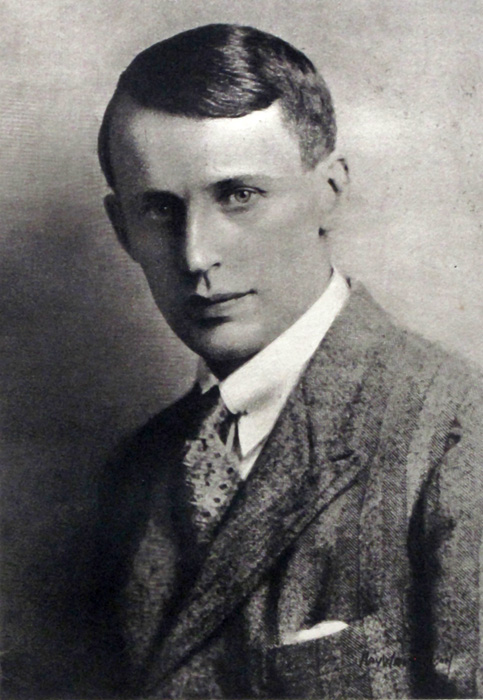
\includegraphics[scale=.4]{Ressources/G.P_Thomson.jpg} 
 		\item G.P. Thomson 
 	\end{itemize**} \\
 
  \end{tabular}

\newpage
	\section{L'expérience de J. J. Thomson}
Lors de ses recherches dans son laboratoire de Cambridge, Thomson conçoit un dispositif dans lequel un faisceau d'électrons est dévié lors de son passage entre deux plaques où règne un champ électrique. La mesure de la déviation du faisceau d'électron lui permet alors de déterminer le rapport $\dfrac{e}{m_e}$.\\
L'étude suivante porte sur le mouvement d'un électron du faisceau qui pénètre entre deux plaques parallèles et horizontales $P_1$ et $P_2$, dans une zone où règne un champ électriques $\vec{E}$ supposé uniforme et perpendiculaire aux deux plaques.\\

\begin{multicols}{2}
\begin{tikzpicture}
	\draw (0,-2)--(6,-2)--(6,2)--(0,2)--cycle;
	\draw[-Stealth] (0,0) to (6.5,0);
	\draw[-Stealth] (0,0) to (0,2.5);
	
	\draw[-Stealth,line width = 1pt] (0,0) to (1,0);
	\draw[-Stealth,line width = 1pt] (0,0) to (0,1);
	 
	\draw[Stealth-Stealth] (0,-2.5) to (6,-2.5);
	
	\node[above, blue] (v0) at (1,.1){$\vv{v_0}$};
	\node[below] (L) at (3,-2.50){$L$};
	\node[below left] (H) at (6,0){$H$};
	\node[left] (O) at (0,0){$O$};
	\node[right] (P1) at (6,2){$P_1$};
	\node[right] (P2) at (6,-2){$P_2$};
	\node[left] (j) at (0,.5){$\vec{j}$};
	\node[below] (i) at (.5,0){$\vec{i}$};
	
	\draw[-Stealth,line width = 1pt, blue] (0,0) to (2,0);
	\draw[domain=0:6, thick, blue] plot(\x,0.04*\x^2);
	\node[right] (S) at (6,1.44){$S$};
	\node[below right] (x) at (6.5,0){$x$};
	\node[above left] (y) at (0,2.5){$y$};	
\end{tikzpicture}
\columnbreak

 À l'instant $t=0~s$, l'électron arrive en un point o avec une vitesse horizontale $\vec{v_0}$.\\
 
 La trajectoire de l'électron dans un repère ($O$, $x$, $y$) est fournie ci-contre.\\
 
L'électron de masse $m_e$ et de charge $q=-e$ dont le mouvement est étudié dans le référentiel terrestre supposé galiléen, est soumis à la seule force électrostatique $\vec{F_e}$. 
\end{multicols}

\begin{enumerate}
\setcounter{enumi}{4}
	\item Sur la figure, représenter sans soucis d'échelle et en justifiant les tracés :
	\begin{itemize*}
		\item le vecteur force $\vec{F_e}$ en un point de la trajectoire de l'électron
		\item le vecteur champ électrique $\vec{E}$ en un point quelconque situé entre les plaques $P_1$ et $P_2$.
	\end{itemize*}
 	\item En utilisant la deuxième loi de Newton, déterminer les équations horaires $x(t)$ et $y(t)$ du mouvement de l'électron.
 	\item Vérifier que la trajectoire de l'électron a pour équation : 
 	$$y = \dfrac{e \cdot E}{2 m_e v_0^2} \cdot x^2$$
 	\item À la sortie de la zone entre les plaques $P_1$ et $P_2$, l'électron a subi une déviation verticale $SH$ comme l'indique le schéma. On mesure $SH = y_S$ = \SI{2,0E-2}{m}. Déterminer, dans cette expérience, la valeur du rapport $\dfrac{e}{m_E}$ de l'électron. Conclure.
\end{enumerate}
\textbf{Données :}
\begin{itemize*}
	\item Longueur des plaques : $L$ = \SI{9,0 E-2}{m}
	\item Vitesse initiale de l'élection : $v_0$ = \SI{2,4E7}{\meter\per\second}
	\item Valeur du champ électrique : $E$ = \SI{1,6E4}{\volt\per\meter}
\end{itemize*}


  \end{document}